\documentclass[11pt,a4paper]{article}

\usepackage[utf8]{inputenc}
\usepackage[T1]{fontenc}
\usepackage{newtxtext,newtxmath}
\usepackage[margin=2.3cm]{geometry}
\usepackage{microtype}
\usepackage{graphicx}
\usepackage{booktabs}
\usepackage{tabularx}
\usepackage{float}
\usepackage[font=small,labelfont=bf]{caption}
\usepackage{xcolor}
\usepackage{listings}
\usepackage{enumitem}
\usepackage{titlesec}
\usepackage{fancyhdr}
\usepackage[most]{tcolorbox}
\usepackage{tikz}
\usetikzlibrary{arrows.meta,calc,shapes.geometric}
\usepackage[hidelinks]{hyperref}

% ---------- Idioma (babel-spanish no esta instalado) ----------
\renewcommand{\figurename}{Figura}
\renewcommand{\tablename}{Tabla}
\renewcommand{\lstlistingname}{Código}

% ---------- Estilo general ----------
\definecolor{acento}{RGB}{31,58,104}
\definecolor{codigofondo}{RGB}{247,247,247}
\definecolor{comentario}{RGB}{110,110,110}
\definecolor{clave}{RGB}{31,58,140}

\titleformat{\section}{\Large\bfseries\color{acento}}{\thesection.}{0.6em}{}
\titleformat{\subsection}{\large\bfseries\color{acento}}{\thesubsection}{0.6em}{}
\titlespacing*{\section}{0pt}{1.4em}{0.6em}
\titlespacing*{\subsection}{0pt}{1.1em}{0.4em}

\pagestyle{fancy}
\fancyhf{}
\fancyhead[L]{\small Arquitectura de Computadoras --- Proyecto 2}
\fancyhead[R]{\small Entrega E1}
\fancyfoot[C]{\small \thepage}
\renewcommand{\headrulewidth}{0.4pt}

\setlist[itemize]{nosep, leftmargin=*, topsep=2pt, partopsep=0pt}
\setlist[enumerate]{nosep, leftmargin=*, topsep=2pt, partopsep=0pt}
\setlength{\parskip}{5pt}
\setlength{\parindent}{0pt}
\widowpenalty=10000
\clubpenalty=10000

\newcommand{\sig}[1]{\texttt{\detokenize{#1}}}

\newtcolorbox{nota}[1]{colback=acento!4, colframe=acento!70, fonttitle=\bfseries\small,
  title={#1}, boxrule=0.6pt, arc=2pt, left=6pt, right=6pt, top=4pt, bottom=4pt}

\lstdefinelanguage{rvasm}{
  morekeywords={addi,add,sub,and,or,xor,slt,andi,ori,xori,lw,sw,beq,jal,jalr,nop},
  morecomment=[l]{\#}, sensitive=true
}
\lstdefinestyle{base}{
  basicstyle=\ttfamily\footnotesize,
  keywordstyle=\color{clave}\bfseries,
  commentstyle=\color{comentario}\itshape,
  columns=fullflexible, keepspaces=true,
  literate={á}{{\'a}}1 {é}{{\'e}}1 {í}{{\'i}}1 {ó}{{\'o}}1 {ú}{{\'u}}1 {ñ}{{\~n}}1
}
% Listados en caja tcolorbox: nunca se cortan entre paginas
\tcbuselibrary{listings}
\tcbset{codigo/.style={listing only, colback=codigofondo, colframe=black!15, boxrule=0.4pt, arc=1pt,
  left=4pt, right=4pt, top=1pt, bottom=1pt, before skip=6pt, after skip=8pt}}
\newtcblisting{asm}{codigo, listing options={style=base, language=rvasm}}
\newtcblisting{vlog}{codigo, listing options={style=base, language=Verilog}}
\newtcblisting{cmd}{codigo, listing options={style=base}}

% ---------- Estilos de diagramas ----------
\tikzset{
  blk/.style={draw, thick, fill=white, align=center, font=\footnotesize, inner sep=2pt},
  preg/.style={draw, thick, fill=acento!12, minimum width=0.38cm},
  mux/.style={draw, thick, fill=white, rounded corners=4pt, minimum width=0.38cm, minimum height=1.0cm, inner sep=0pt},
  ctl/.style={draw, thick, ellipse, fill=orange!10, align=center, font=\footnotesize, inner sep=1pt, minimum width=1.7cm, minimum height=0.75cm},
  hz/.style={draw, thick, fill=red!7, align=center, font=\footnotesize},
  dat/.style={-{Stealth[length=2mm]}, thick},
  fwd/.style={-{Stealth[length=2mm]}, thick, blue!60!black},
  hzl/.style={-{Stealth[length=1.6mm]}, red!60!black, dashed},
  lbl/.style={font=\scriptsize, inner sep=1.5pt},
  futuro/.style={draw, thick, dashed, gray, fill=gray!7, align=center, font=\footnotesize, text=gray!60!black},
  dot/.style={circle, fill, inner sep=1.2pt}
}

\begin{document}

% =====================================================================
% Encabezado
% =====================================================================
\begin{center}
  {\LARGE\bfseries\color{acento} Proyecto 2 --- Entrega E1\par}
  \vspace{10pt}
  Aedo Farge, Gian Franco\\
  Colque Ordoñez, Patrick Fabrizio\\
  Sander's Arana, Ralfh Krishna Karl\par
  \vspace{8pt}
  {\small Arquitectura de Computadoras, noviembre de 2026\par}
\end{center}

\begin{nota}{Resumen}
Implementamos un pipeline RV32I de cinco etapas con forwarding, stalling y flushing, y lo verificamos con cuatro programas de prueba que pasan sus testbenches automáticos. En el camino encontramos y corregimos un error por el que \sig{jalr} no anulaba las instrucciones del camino incorrecto. Sobre ese pipeline empezamos la arquitectura Dual-Issue: el procesador ya lee y decodifica dos instrucciones por ciclo y tiene un Register File de cuatro lecturas y dos escrituras. También quedaron instanciados el registro ID/EX y la ALU de la segunda vía. Por ahora el procesador sigue emitiendo una instrucción por ciclo, en orden.
\end{nota}

% =====================================================================
\section{Organización del trabajo}
% =====================================================================

El proyecto termina comparando tres arquitecturas: (A) el pipeline Single-Issue, (B) el Dual-Issue y (C) el Dual-Issue optimizado. Para que esa comparación sea justa, cada arquitectura se conserva como una versión separada del código y ninguna modifica a la anterior. En esta entrega hay dos: la versión Single-Issue, que es la arquitectura A ya terminada, y la versión Dual-Issue, que parte de ella y contiene el avance hacia B. Todas las waveforms de este informe se obtuvieron simulando los testbenches incluidos en el código, con un reloj de 10~ns; el reset se desactiva a los 22~ns.

% =====================================================================
\section{El pipeline de cinco etapas}
% =====================================================================

Cada instrucción pasa por cinco etapas separadas por registros de pipeline (Tabla~\ref{tab:etapas}). Como en cada ciclo hay hasta cinco instrucciones avanzando a la vez, en el caso ideal se termina una instrucción por ciclo (CPI~$=1$). El procesador soporta \sig{add}, \sig{sub}, \sig{and}, \sig{or}, \sig{xor}, \sig{slt}, sus versiones con inmediato, \sig{lw}, \sig{sw}, \sig{beq}, \sig{jal} y \sig{jalr}.

\begin{table}[htbp]
\centering
\caption{Etapas del pipeline.}
\label{tab:etapas}
\begin{tabularx}{\textwidth}{l X l}
\toprule
\textbf{Etapa} & \textbf{Qué hace} & \textbf{Registro} \\
\midrule
IF  & Lee la instrucción en \sig{PCF} y calcula \sig{PC+4}. & IF/ID \\
ID  & Decodifica, lee \sig{rs1} y \sig{rs2} del Register File y extiende el inmediato. & ID/EX \\
EX  & Opera la ALU, calcula el destino del salto y decide si se toma (\sig{PCSrcE}). & EX/MEM \\
MEM & \sig{lw} lee y \sig{sw} escribe en la memoria de datos. & MEM/WB \\
WB  & Elige el resultado (ALU, dato leído o \sig{PC+4}) y lo escribe en el Register File. & --- \\
\bottomrule
\end{tabularx}
\end{table}

\subsection{Datapath}

La Figura~\ref{fig:dp-single} muestra el datapath. Las señales llevan como sufijo la etapa donde están (\sig{F}, \sig{D}, \sig{E}, \sig{M}, \sig{W}). Además de datos y control, los registros de pipeline propagan la instrucción completa (\sig{InstrD} a \sig{InstrW}); no la necesita el hardware, pero permite ver en las waveforms en qué etapa está cada instrucción.

\begin{figure}[htbp]
\centering
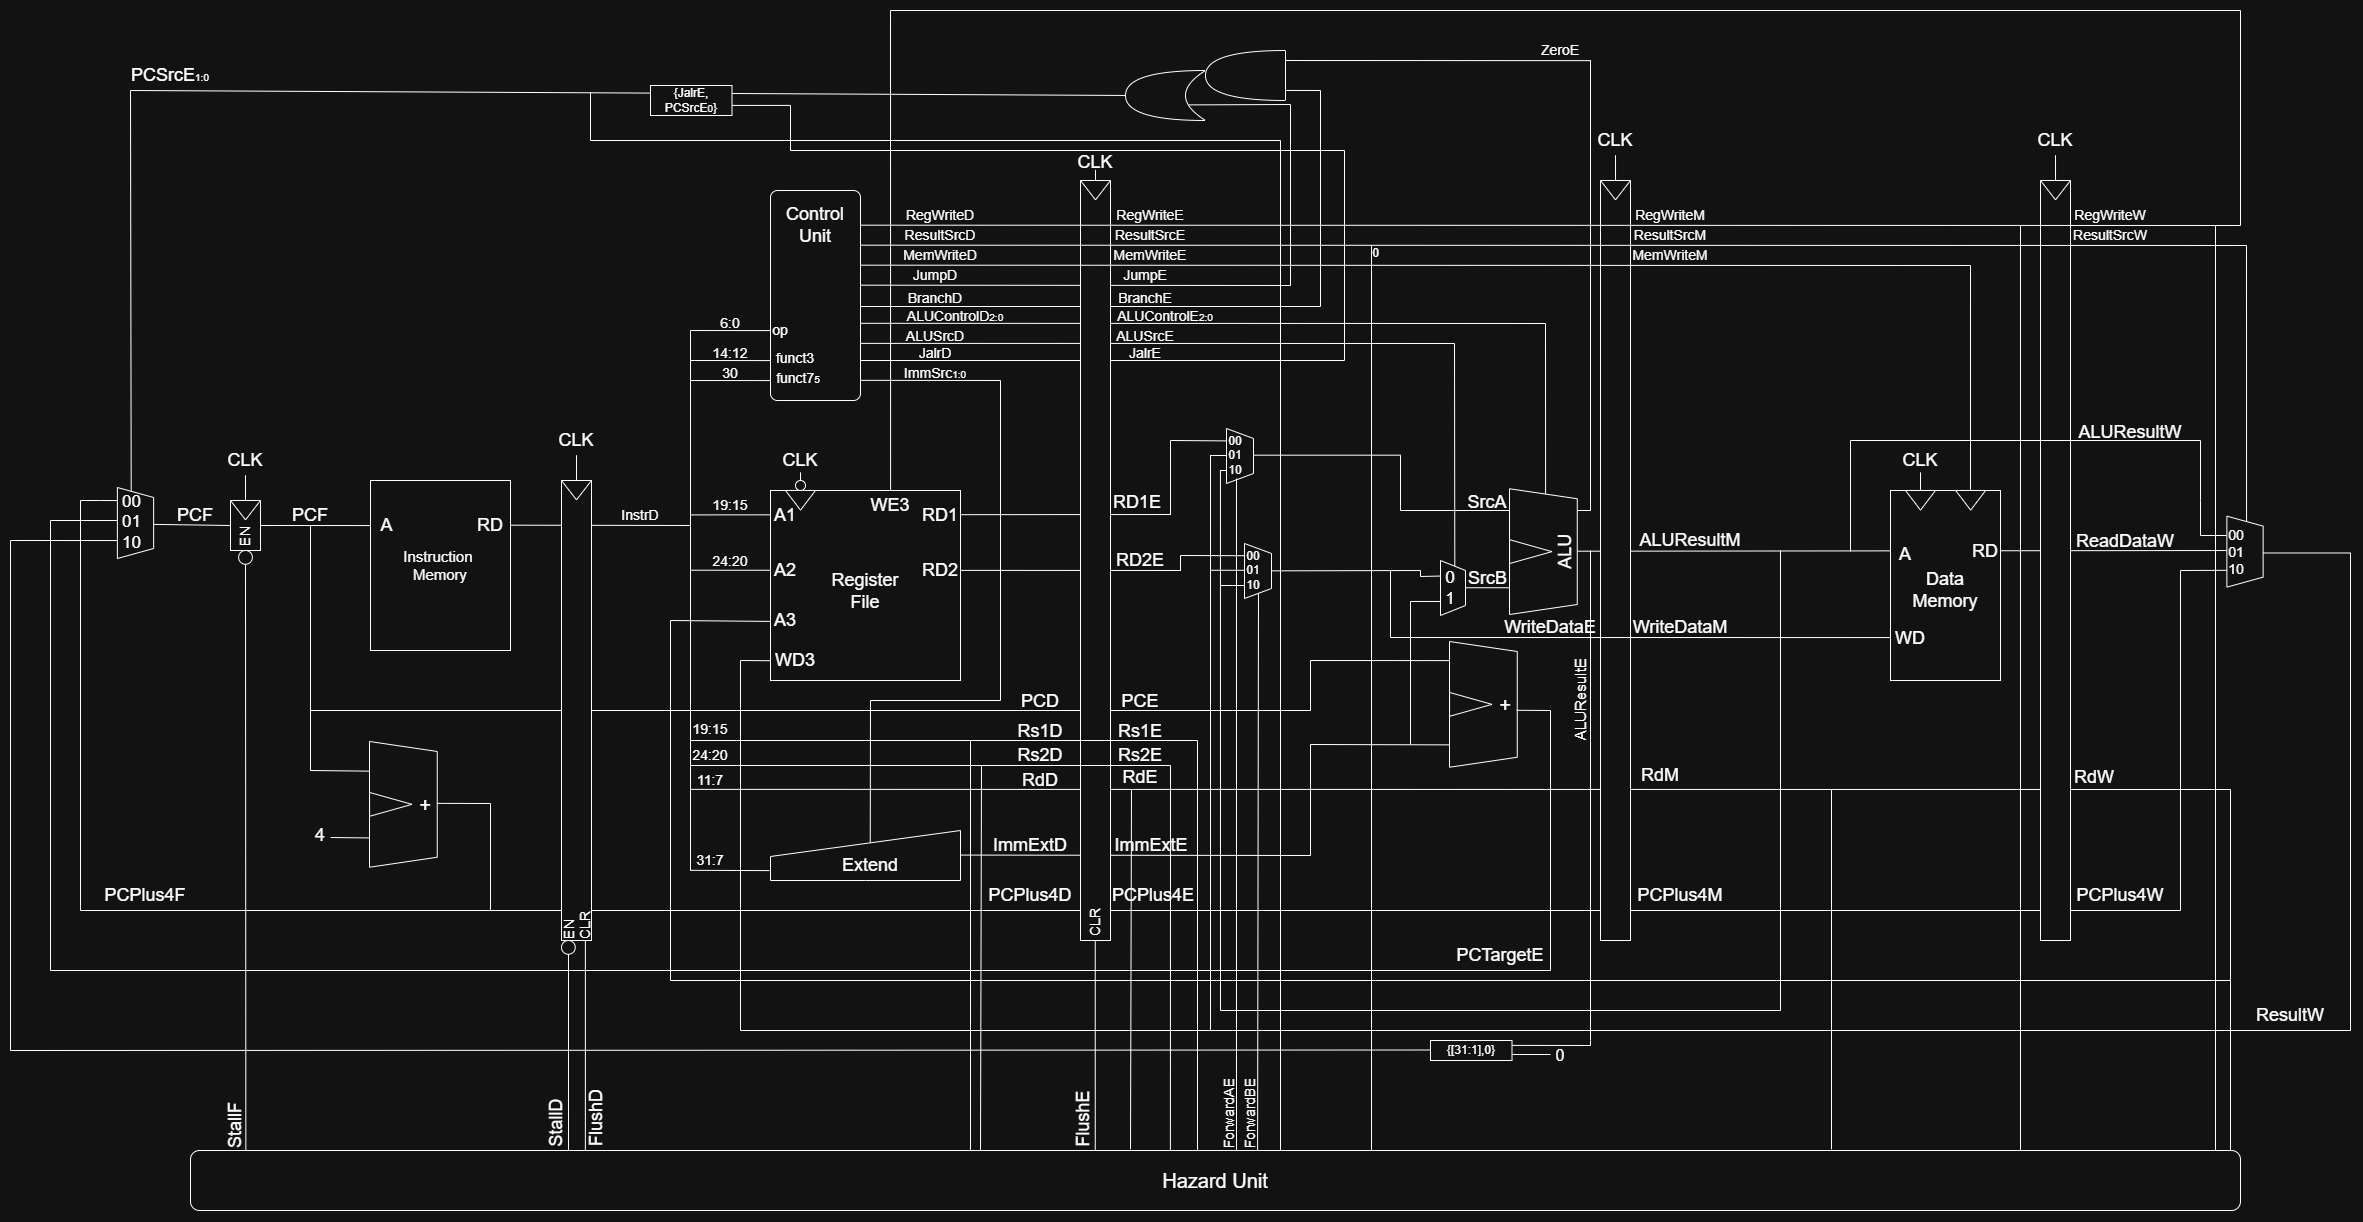
\includegraphics[width=\textwidth]{../img/Pipeline_Single_Issue_Datapath_with_Hazard.jpg}\\[4pt]
\caption{Datapath del pipeline Single-Issue con la Hazard Unit: registros de pipeline, multiplexores de forwarding en EX y señales de stall y flush.}
\label{fig:dp-single}
\end{figure}

El multiplexor del PC tiene tres entradas: \sig{00} para \sig{PC+4}, \sig{01} para el destino de \sig{beq} y \sig{jal} (\sig{PCTargetE}) y \sig{10} para \sig{jalr}, cuyo destino es \sig{ALUResultE} con el bit~0 en cero. El Register File escribe en el flanco de bajada del reloj: así, una instrucción en WB escribe en la primera mitad del ciclo y la que está en ID lee el valor nuevo en la segunda mitad, lo que nos ahorra un caso de forwarding. Cuando el registro IF/ID se anula, se carga un NOP real (\sig{addi x0, x0, 0}) en lugar de ceros, para que el controller nunca decodifique una instrucción inválida.

\subsection{Unidad de control}

El controller decodifica en ID con \sig{maindec} y \sig{aludec} y hace viajar cada señal con su instrucción hasta la etapa donde se usa. \sig{ImmSrc} se consume en ID; \sig{ALUSrc}, \sig{ALUControl}, \sig{Branch}, \sig{Jump} y \sig{Jalr} en EX; \sig{MemWrite} en MEM, y \sig{RegWrite} y \sig{ResultSrc} en WB. El salto se resuelve en EX con \texttt{PCSrcE = \{JalrE, (BranchE \& ZeroE) | JumpE\}}. El registro de control ID/EX se limpia con \sig{FlushE}, de modo que una instrucción anulada no escribe registros ni memoria. Respecto al procesador single-cycle original, añadimos la señal \sig{Jalr} a \sig{maindec} (la palabra de control pasó de 11 a 12 bits) para soportar \sig{jalr}.

% =====================================================================
\section{Hazard Unit}
% =====================================================================

La Hazard Unit (\sig{hazardunit.v}) se encarga de los tres tipos de riesgo del pipeline.

\textbf{Forwarding.} Si un registro fuente de la instrucción en EX es el destino de una instrucción en MEM o WB que escribe en el Register File, se le pasa el valor directamente. MEM tiene prioridad porque contiene el resultado más reciente:

\begin{vlog}
if      ((Rs1E != 0) && (Rs1E == RdM) && RegWriteM) ForwardAE = 2'b10; // desde MEM
else if ((Rs1E != 0) && (Rs1E == RdW) && RegWriteW) ForwardAE = 2'b01; // desde WB
else                                                ForwardAE = 2'b00;
\end{vlog}

\textbf{Stall (load-use).} Un \sig{lw} recién tiene su dato al final de MEM. Si la instrucción que le sigue lo necesita, se congelan el PC y el registro IF/ID durante un ciclo y se ingresa una burbuja en EX:

\begin{vlog}
assign lwStall = ResultSrcE0 & (RdE != 5'b0) & ((Rs1D == RdE) | (Rs2D == RdE));
assign StallF  = lwStall;
assign StallD  = lwStall;
\end{vlog}

\textbf{Flush.} Para instrucciones del formato B o de salto, el salto se decide en EX, pero para entonces ya entraron dos instrucciones (en IF e ID). Si el salto se toma, ambas se anulan, realizando el Flush con los registros IF/ID e ID/EX:

\begin{vlog}
assign FlushD = |PCSrcE;
assign FlushE = lwStall | (|PCSrcE);
\end{vlog}

\begin{nota}{Error corregido: \sig{jalr} no hacía flush}
La versión original tenía \sig{assign FlushD = PCSrcE;}. \sig{PCSrcE} es de 2~bits y \sig{FlushD} de 1, así que Verilog se quedaba solo con el bit menos significativo. Para \sig{jalr} (\sig{PCSrcE = 10}) eso daba \sig{FlushD = 0}, y las dos instrucciones siguientes se ejecutaban aunque no debían. Lo corregimos con la reducción OR (\sig{|PCSrcE}), que vale 1 ante cualquier salto tomado. El Programa~4 lo comprueba: con la versión anterior, \sig{x14} y \sig{x15} terminaban en 99; con la corregida quedan en~0. También agregamos \sig{RdE != 0} a \sig{lwStall}, porque un \sig{lw} hacia \sig{x0} no debería frenar el pipeline.
\end{nota}

% =====================================================================
\section{Programas de prueba}
% =====================================================================

Cada programa tiene su código Assembly, su archivo \sig{.mem} (verificado contra el ensamblador RISC-V) y un testbench que revisa por sí solo los registros, la memoria y la cantidad de stalls y flushes. La Tabla~\ref{tab:resultados} resume lo obtenido; en las secciones siguientes explicamos cada waveform.

\begin{table}[htbp]
\centering
\caption{Resultados de los programas de prueba sobre el pipeline Single-Issue.}
\label{tab:resultados}
\begin{tabular}{l l l c}
\toprule
\textbf{Programa} & \textbf{Qué prueba} & \textbf{Qué se observa} & \textbf{Testbench} \\
\midrule
1 --- ISA        & Todas las instrucciones, sin dependencias & Sin forwarding, stall ni flush & PASS \\
2 --- Forwarding & Cadena de dependencias RAW     & 4 ciclos con forwarding & PASS \\
3 --- Stalling   & Dependencia load-use           & 1 stall & PASS \\
4 --- Flushing   & \sig{beq}, \sig{jal}, \sig{jalr} & 3 flushes & PASS \\
\bottomrule
\end{tabular}
\end{table}

\subsection{Programa 1: instrucciones sin dependencias}

Este programa recorre todas las instrucciones que soporta el procesador y las ordena para que ninguna necesite a la Hazard Unit: cada instrucción que produce un valor está al menos a tres instrucciones de la que lo usa, distancia a la que el Register File ya tiene el dato gracias a la escritura en flanco de bajada. \sig{jal}, \sig{jalr} y un \sig{beq} tomado no pueden probarse aquí, porque siempre provocan un flush; esos se verifican en el Programa~4. El testbench comprueba los registros \sig{x1} a \sig{x18}, las dos palabras escritas en memoria y que durante todo el programa no haya ningún forwarding, stall ni flush.

\begin{asm}
addi x4, x0, 3      # x4 = 3
addi x1, x0, 12     # x1 = 12
addi x2, x0, 5      # x2 = 5
addi x3, x0, 8      # x3 = 8
                    # 4 NOP
add  x5, x1, x2     # x5 = 17
sub  x6, x3, x4     # x6 = 5
and  x7, x1, x3     # x7 = 8
or   x8, x2, x4     # x8 = 7
xor  x9, x1, x2     # x9 = 9
slt  x10, x4, x2    # x10 = 1   (3 < 5)
addi x11, x0, -5    # x11 = -5
andi x12, x1, 6     # x12 = 4   (12 & 6)
ori  x13, x2, 8     # x13 = 13  (5 | 8)
xori x14, x3, 15    # x14 = 7   (8 ^ 15)
slti x15, x2, 7     # x15 = 1   (5 < 7)
sw   x1, 0(x0)      # Mem[0] = 12
sw   x2, 4(x0)      # Mem[1] = 5
lw   x16, 0(x0)     # x16 = 12
lw   x17, 4(x0)     # x17 = 5
                    # 3 NOP
beq  x16, x17, salto  # 12 != 5: no se toma
addi x18, x0, 1     # x18 = 1
salto:
\end{asm}

\begin{figure}[htbp]
\centering
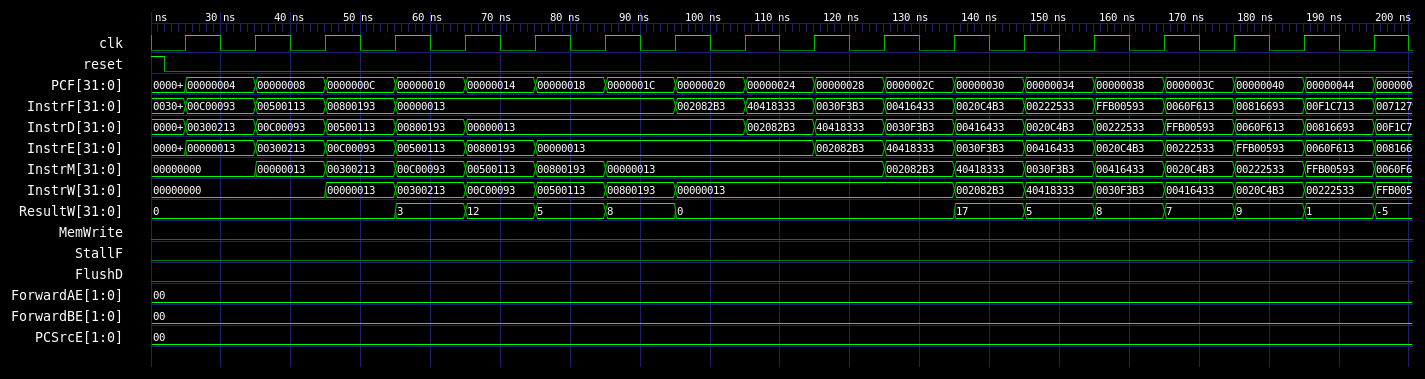
\includegraphics[width=\textwidth]{../img/prog1_isa_a.png}\\[4pt]
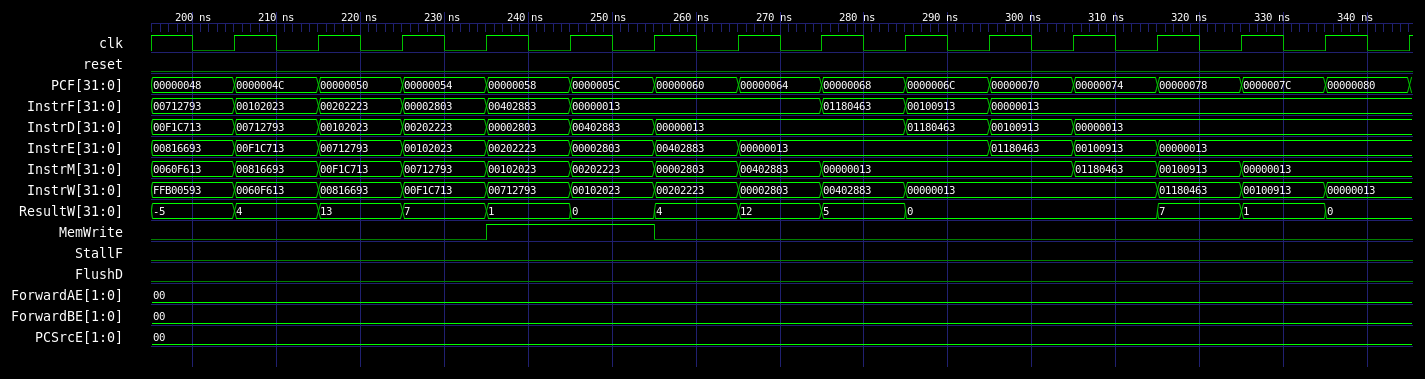
\includegraphics[width=\textwidth]{../img/prog1_isa_b.png}
\caption{Programa 1. Arriba, de 20 a 200~ns; abajo, de 195 a 345~ns.}
\label{fig:p1}
\end{figure}

En la Figura~\ref{fig:p1} se ve el caso ideal del pipeline: cada instrucción baja en diagonal de \sig{InstrF} a \sig{InstrW}, una etapa por ciclo, y el PC avanza de 4 en 4 sin detenerse. \sig{StallF}, \sig{FlushD}, \sig{ForwardAE}, \sig{ForwardBE} y \sig{PCSrcE} se mantienen en 0 durante todo el programa, así que la Hazard Unit nunca interviene. \sig{ResultW} muestra los valores en el orden en que se escriben: 3, 12, 5 y 8 de la inicialización (60--90~ns); 17, 5, 8, 7, 9 y 1 de las instrucciones tipo~R, incluido el \sig{slt} (140--190~ns), y $-5$, 4, 13, 7 y 1 de las instrucciones con inmediato (200--240~ns).

La parte de memoria está en la captura inferior. \sig{MemWrite} sube durante dos ciclos, entre los 235 y 255~ns: son los dos \sig{sw}, que escriben 12 en \sig{Mem[0]} y 5 en \sig{Mem[1]}. A los 270 y 280~ns, \sig{ResultW} muestra 12 y 5, los valores que los \sig{lw} leyeron de esas mismas direcciones. El \sig{beq} llega a EX a los 300~ns; como $12 \neq 5$, \sig{PCSrcE} sigue en \sig{00}, no hay flush, y \sig{addi x18} escribe su 1 a los 330~ns. Los valores 0 y 4 de \sig{ResultW} hacia los 250~ns son las direcciones que calcularon los \sig{sw}, y el 7 de los 320~ns es la resta $12-5$ del \sig{beq}; ninguno se escribe, porque esas instrucciones tienen \sig{RegWrite = 0}.

\subsection{Programa 2: forwarding}

\begin{asm}
addi x1, x0, 5      # x1 = 5
addi x2, x0, 10     # x2 = 10
add  x3, x1, x2     # x3 = 15   (x1 desde WB, x2 desde MEM)
sub  x4, x3, x1     # x4 = 10   (x3 desde MEM)
add  x5, x4, x3     # x5 = 25   (x4 desde MEM, x3 desde WB)
add  x6, x5, x4     # x6 = 35   (x5 desde MEM, x4 desde WB)
\end{asm}

\begin{figure}[htbp]
\centering
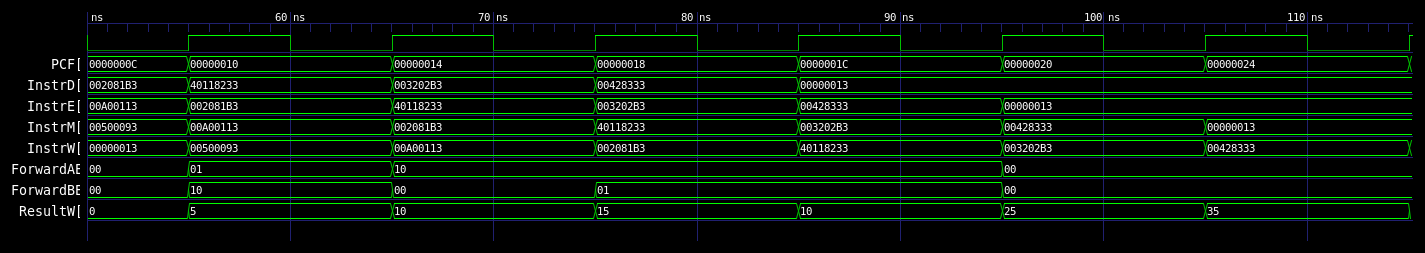
\includegraphics[width=\textwidth]{../img/prog2_forwarding.png}
\caption{Programa 2, de 50 a 115~ns.}
\label{fig:p2}
\end{figure}

Aquí cada instrucción necesita el resultado de la anterior antes de que llegue al Register File. La Tabla~\ref{tab:p2} resume lo que hace el forwarding en cada ciclo de la Figura~\ref{fig:p2}. Ninguna instrucción se detiene: sin forwarding, cada una habría esperado dos ciclos. \sig{ResultW} confirma los valores 15, 10, 25 y 35 entre los 80 y 110~ns.

\begin{table}[htbp]
\centering
\caption{Forwarding observado en el Programa 2.}
\label{tab:p2}
\begin{tabular}{c l c c l}
\toprule
\textbf{Tiempo} & \textbf{En EX} & \sig{ForwardAE} & \sig{ForwardBE} & \textbf{De dónde vienen los operandos} \\
\midrule
60~ns & \sig{add x3, x1, x2} & 01 & 10 & \sig{x1} desde WB, \sig{x2} desde MEM \\
70~ns & \sig{sub x4, x3, x1} & 10 & 00 & \sig{x3} desde MEM \\
80~ns & \sig{add x5, x4, x3} & 10 & 01 & \sig{x4} desde MEM, \sig{x3} desde WB \\
90~ns & \sig{add x6, x5, x4} & 10 & 01 & \sig{x5} desde MEM, \sig{x4} desde WB \\
\bottomrule
\end{tabular}
\end{table}

\subsection{Programa 3: stalling por load-use}

\begin{asm}
addi x1, x0, 0      # x1 = 0
addi x2, x0, 10     # x2 = 10
sw   x2, 0(x1)      # Mem[0] = 10
lw   x3, 0(x1)      # x3 = 10
add  x4, x3, x2     # x4 = 20   <- usa x3 justo despues del lw: stall
sub  x5, x4, x2     # x5 = 10
add  x6, x5, x3     # x6 = 20
\end{asm}

\begin{figure}[htbp]
\centering
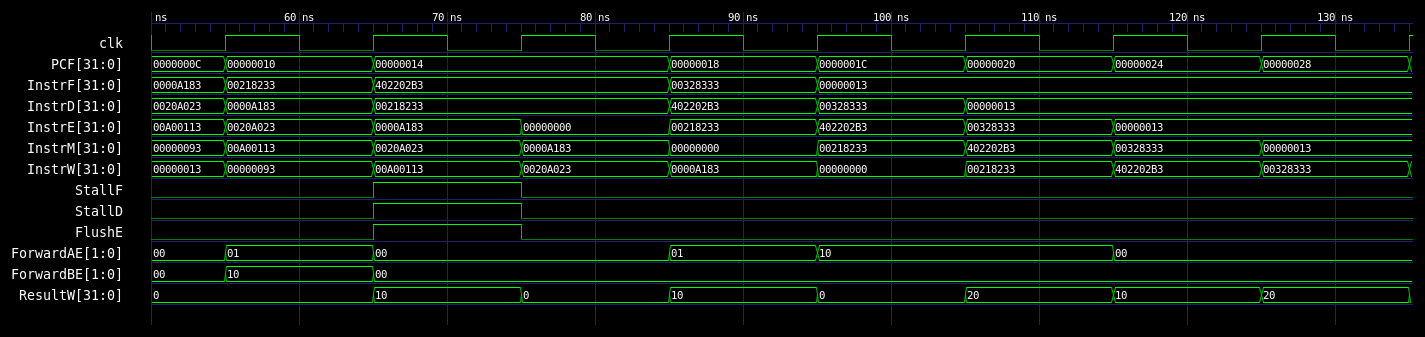
\includegraphics[width=\textwidth]{../img/prog3_stalling.png}
\caption{Programa 3, de 50 a 135~ns.}
\label{fig:p3}
\end{figure}

La Figura~\ref{fig:p3} muestra el único stall del programa. A los 60~ns, el \sig{sw} recibe por forwarding desde MEM el dato que va a guardar (\sig{ForwardBE = 10}). A los 70~ns el \sig{lw x3} está en EX y el \sig{add x4, x3, x2} en ID; como \sig{x3} recién estará listo al final de MEM, la Hazard Unit levanta a la vez \sig{StallF}, \sig{StallD} y \sig{FlushE}. El efecto se ve claro a los 80~ns: \sig{PCF} sigue en \sig{0x14} e \sig{InstrD} sigue siendo el \sig{add}, porque ambos quedaron congelados, mientras \sig{InstrE} vale 0, que es la burbuja insertada.

Un ciclo después, a los 90~ns, el \sig{add} entra a EX y toma \sig{x3 = 10} desde WB (\sig{ForwardAE = 01}), porque el \sig{lw} ya leyó la memoria. Las dos instrucciones siguientes obtienen su operando desde MEM (\sig{ForwardAE = 10}) sin más esperas. Un ciclo de stall es el costo mínimo de una dependencia load-use en este pipeline.

\subsection{Programa 4: flushing}

\begin{asm}
      addi x1, x0, 5
      addi x2, x0, 5
      addi x3, x0, 7
      beq  x1, x3, t1     # NO se toma (5 != 7)
      addi x4, x0, 1      # x4 = 1
      beq  x1, x2, t1     # se toma -> flush
      addi x5, x0, 99     # anulada
      addi x6, x0, 99     # anulada
t1:   addi x7, x0, 2
      jal  x8, t2         # x8 = 40 -> flush
      addi x9, x0, 99     # anulada
      addi x10, x0, 99    # anulada
t2:   addi x11, x0, 3
      addi x12, x0, 68
      jalr x13, 0(x12)    # x13 = 60 -> flush
      addi x14, x0, 99    # anulada
      addi x15, x0, 99    # anulada
t3:   addi x16, x0, 4
      sw   x16, 0(x0)
fin:  beq  x0, x0, fin
\end{asm}

\begin{figure}[htbp]
\centering
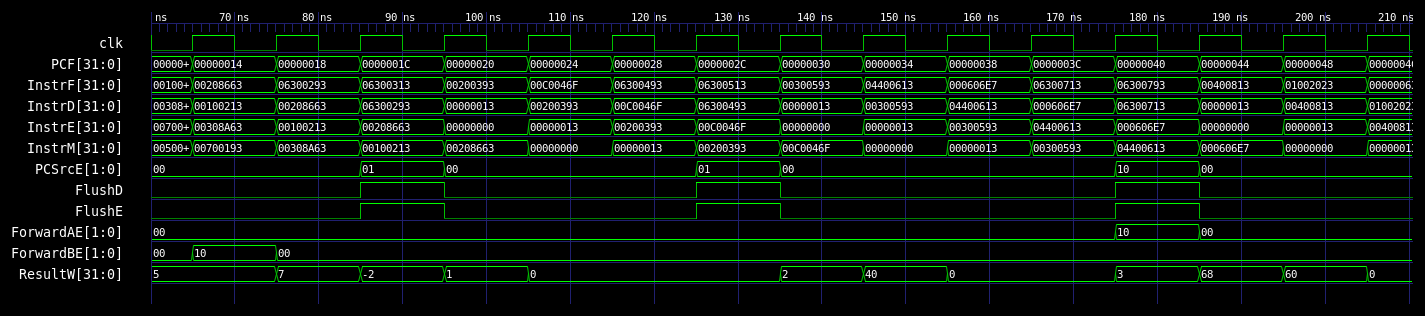
\includegraphics[width=\textwidth]{../img/prog4_flushing.png}
\caption{Programa 4, de 60 a 210~ns.}
\label{fig:p4}
\end{figure}

El programa recorre los tres tipos de salto. En la Figura~\ref{fig:p4}, a los 70~ns el primer \sig{beq} está en EX y recibe \sig{x3} por forwarding (\sig{ForwardBE = 10}); como $5 \neq 7$, \sig{PCSrcE} queda en \sig{00} y no pasa nada: \sig{addi x4} sigue su camino.

A los 90~ns el segundo \sig{beq} sí se toma. \sig{PCSrcE} pasa a \sig{01} y se activan \sig{FlushD} y \sig{FlushE}, que anulan las dos \sig{addi ..., 99} que estaban en ID e IF. En el ciclo siguiente se ve el resultado: \sig{InstrD} es un NOP, \sig{InstrE} vale 0 y \sig{PCF} ya apunta a \sig{0x20} (\sig{t1}). El \sig{jal} de los 130~ns se comporta igual, y a los 150~ns \sig{ResultW} muestra el 40 que se guarda en \sig{x8} como dirección de retorno.

El caso más interesante es el \sig{jalr} de los 180~ns. Recibe \sig{x12 = 68} por forwarding desde MEM (\sig{ForwardAE = 10}), pone \sig{PCSrcE = 10} y esta vez sí provoca el flush, que es justamente lo que fallaba antes de la corrección. A los 190~ns el PC ya está en \sig{0x44} (\sig{t3}) y a los 200~ns \sig{ResultW} muestra el 60 de \sig{x13}.

El $-2$ que aparece en \sig{ResultW} hacia los 90~ns no es un error: es la resta $5-7$ que hizo el \sig{beq} no tomado al llegar a WB, y no se escribe en ningún registro porque \sig{beq} tiene \sig{RegWrite = 0}. Cada salto tomado cuesta dos ciclos, uno por cada instrucción anulada.

% =====================================================================
\section{Primeros pasos hacia Dual-Issue}
% =====================================================================

En esta entrega construimos la parte frontal del procesador Dual-Issue: leer y decodificar dos instrucciones por ciclo. La ejecución en paralelo (Issue Unit y segunda ALU) queda para E2. La Figura~\ref{fig:dp-dual} resume los cambios.

\textbf{Dual Fetch.} A la memoria de instrucciones le agregamos un segundo puerto de lectura: \sig{rd} entrega la instrucción en \sig{PC} y \sig{rd1} la de \sig{PC+4}. Como en cada lectura llega un par, el PC avanza de 8 en 8. El PC se actualiza cuando el par que está en Decode ya terminó de emitirse o cuando hay un salto tomado.

\textbf{Dual Decode.} El registro IF/ID ahora es doble y guarda \sig{InstrD0} (slot~0, la instrucción más antigua), \sig{InstrD1} (slot~1) y el PC base del par. El controller tiene dos decodificadores (dos \sig{maindec} y dos \sig{aludec}) y el datapath dos unidades \sig{extend}, así que ambas instrucciones se decodifican en el mismo ciclo. El Register File pasó a tener cuatro puertos de lectura y dos de escritura: lee \sig{rs1} y \sig{rs2} de las dos instrucciones a la vez. El segundo puerto de escritura ya existe y, si las dos vías escriben el mismo registro, gana la vía~1 por ser la instrucción más joven; lo conectaremos en E2.

\textbf{Módulos de la vía 1.} También instanciamos el registro ID/EX de la vía 1 (\sig{regE1}, con los operandos, el inmediato y el control del slot~1) y su ALU (\sig{alu1}), con su propio multiplexor de \sig{ALUSrc}. En esta entrega la señal \sig{Issue1D} está fija en 0, de modo que ese registro se limpia en cada ciclo y la vía 1 solo procesa burbujas. En E2 la Issue Unit pondrá \sig{Issue1D} en 1 cuando las dos instrucciones del par puedan salir juntas.

\textbf{Emisión.} Como E1 todavía no pide ejecutar dos instrucciones a la vez, emitimos una por ciclo y en orden. La señal \sig{SelD} elige el slot: con \sig{SelD = 0} sale la instrucción más antigua del par y con \sig{SelD = 1} la más joven; después entra el siguiente par. A EX pasan el control y los operandos del slot elegido. Esta idea de guardar la instrucción más joven para el ciclo siguiente es la base del reagrupamiento que hará la Issue Unit en E2. Ante un salto tomado se limpia el par en Decode, y si el salto estaba en el slot~0, la instrucción del slot~1 se anula con \sig{FlushE}.

\begin{figure}[htbp]
\centering
\resizebox{\textwidth}{!}{%
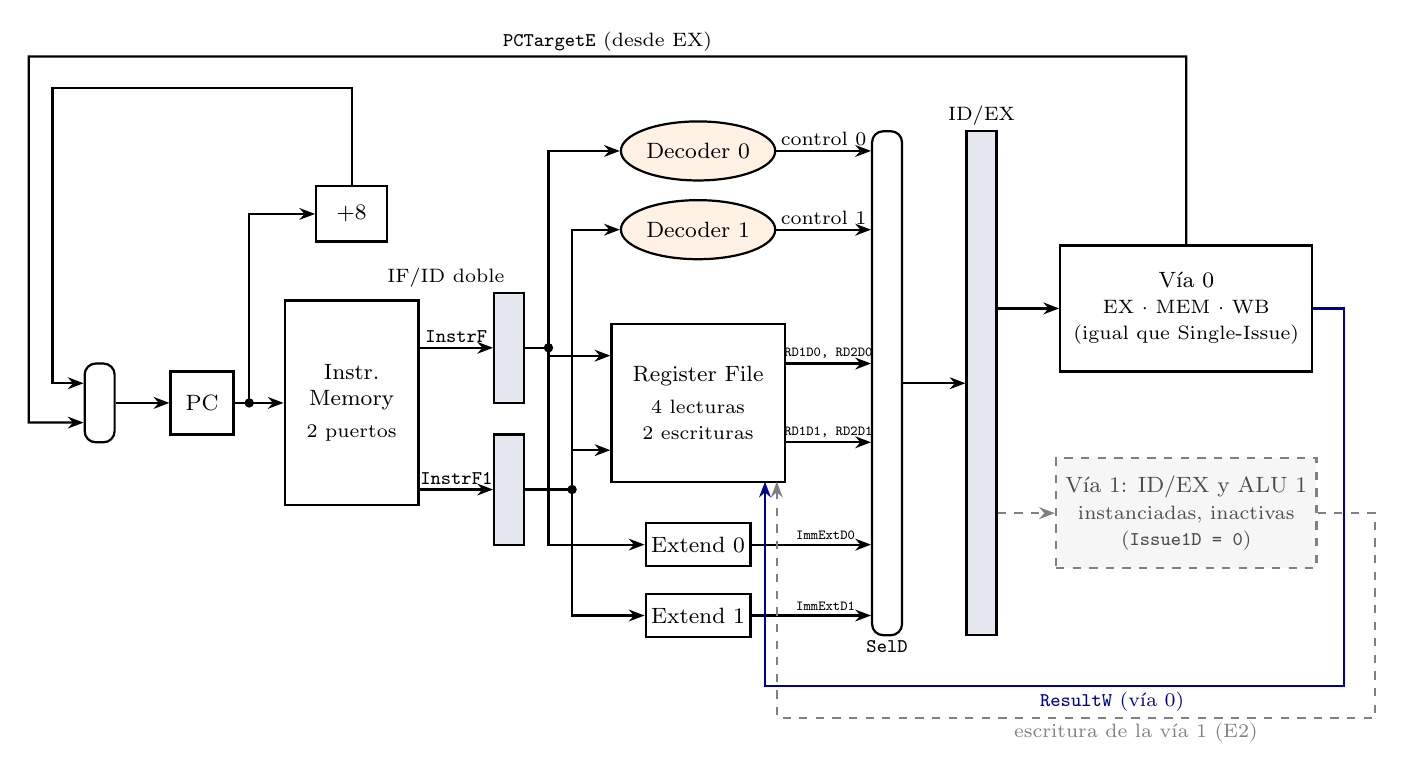
\begin{tikzpicture}[x=1cm,y=1cm]
  % --- fetch ---
  \node[mux] (pcmux) at (0,3.0) {};
  \node[blk, minimum width=0.8cm, minimum height=0.8cm] (pc) at (1.3,3.0) {PC};
  \node[blk, minimum width=1.7cm, minimum height=2.6cm] (imem) at (3.2,3.0) {Instr.\\Memory\\[2pt]\scriptsize 2 puertos};
  \node[blk, minimum width=0.9cm, minimum height=0.7cm] (add8) at (3.2,5.4) {$+8$};
  % --- IF/ID doble ---
  \node[preg, minimum height=1.4cm] (ifid0) at (5.2,3.7) {};
  \node[preg, minimum height=1.4cm] (ifid1) at (5.2,1.9) {};
  \node[lbl, above left] at (ifid0.north) {IF/ID doble};
  % --- decode ---
  \node[ctl, minimum width=1.9cm] (dec0) at (7.6,6.2) {Decoder 0};
  \node[ctl, minimum width=1.9cm] (dec1) at (7.6,5.2) {Decoder 1};
  \node[blk, minimum width=2.2cm, minimum height=2.0cm] (rf) at (7.6,3.0) {Register File\\[2pt]\scriptsize 4 lecturas\\\scriptsize 2 escrituras};
  \node[blk, minimum width=1.3cm, minimum height=0.55cm] (ext0) at (7.6,1.2) {Extend 0};
  \node[blk, minimum width=1.3cm, minimum height=0.55cm] (ext1) at (7.6,0.3) {Extend 1};
  % --- seleccion y resto ---
  \node[mux, minimum height=6.4cm] (sel) at (10.0,3.25) {};
  \node[lbl, below] at (sel.south) {\sig{SelD}};
  \node[preg, minimum height=6.4cm] (idex) at (11.2,3.25) {};
  \node[lbl, above] at (idex.north) {ID/EX};
  \node[blk, minimum width=3.2cm, minimum height=1.6cm] (via0) at (13.8,4.2) {Vía 0\\\scriptsize EX $\cdot$ MEM $\cdot$ WB\\\scriptsize (igual que Single-Issue)};
  \node[futuro, minimum width=3.2cm, minimum height=1.4cm] (via1) at (13.8,1.6) {Vía 1: ID/EX y ALU 1\\\scriptsize instanciadas, inactivas\\\scriptsize (\sig{Issue1D = 0})};
  % --- conexiones fetch ---
  \draw[dat] (pcmux.east) -- (pc.west);
  \draw[dat] (pc.east) -- (imem.west);
  \draw[dat] (1.9,3.0) node[dot]{} |- (add8.west);
  \draw[dat] (add8.north) -- (3.2,7.0) -- (-0.6,7.0) -- (-0.6,3.25) -- ([yshift=0.25cm]pcmux.west);
  \draw[dat] (via0.north) -- (13.8,7.4) -- node[lbl,above]{\sig{PCTargetE} (desde EX)} (-0.9,7.4) -- (-0.9,2.75) -- ([yshift=-0.25cm]pcmux.west);
  \draw[dat] (imem.east |- ifid0.west) -- node[lbl,above]{\sig{InstrF}} (ifid0.west);
  \draw[dat] (imem.east |- ifid1.west) -- node[lbl,above]{\sig{InstrF1}} (ifid1.west);
  % --- bus del slot 0 (x = 5.7) ---
  \draw[thick] (ifid0.east) -- (5.7,3.7) node[dot]{};
  \draw[dat] (5.7,3.7) |- (dec0.west);
  \draw[dat] (5.7,3.6) |- ([yshift=0.6cm]rf.west);
  \draw[dat] (5.7,3.7) |- (ext0.west);
  % --- bus del slot 1 (x = 6.0) ---
  \draw[thick] (ifid1.east) -- (6.0,1.9) node[dot]{};
  \draw[dat] (6.0,1.9) |- (dec1.west);
  \draw[dat] (6.0,1.9) |- ([yshift=-0.6cm]rf.west);
  \draw[dat] (6.0,1.9) |- (ext1.west);
  % --- hacia el mux de seleccion ---
  \draw[dat] (dec0.east) -- node[lbl,above]{control 0} (dec0.east -| sel.west);
  \draw[dat] (dec1.east) -- node[lbl,above]{control 1} (dec1.east -| sel.west);
  \draw[dat] ([yshift=0.5cm]rf.east) -- node[lbl,above,pos=0.5,font=\tiny]{\sig{RD1D0, RD2D0}} ([yshift=0.5cm]rf.east -| sel.west);
  \draw[dat] ([yshift=-0.5cm]rf.east) -- node[lbl,above,pos=0.5,font=\tiny]{\sig{RD1D1, RD2D1}} ([yshift=-0.5cm]rf.east -| sel.west);
  \draw[dat] (ext0.east) -- node[lbl,above,pos=0.62,font=\tiny]{\sig{ImmExtD0}} (ext0.east -| sel.west);
  \draw[dat] (ext1.east) -- node[lbl,above,pos=0.62,font=\tiny]{\sig{ImmExtD1}} (ext1.east -| sel.west);
  \draw[dat] (sel.east) -- (sel.east -| idex.west);
  \draw[dat] (idex.east |- via0.west) -- (via0.west);
  \draw[dat, dashed, gray] (idex.east |- via1.west) -- (via1.west);
  % --- escrituras en el Register File ---
  \draw[fwd] (via0.east) -- (15.8,4.2) -- (15.8,-0.6) -- node[lbl,below,pos=0.4]{\sig{ResultW} (vía 0)} (8.45,-0.6) -- (8.45,2.0);
  \draw[dat, dashed, gray] (via1.east) -- (16.2,1.6) -- (16.2,-1.0) -- node[lbl,below,pos=0.4]{escritura de la vía 1 (E2)} (8.6,-1.0) -- (8.6,2.0);
\end{tikzpicture}}
\caption{Datapath Dual-Issue preliminar. El par se lee y decodifica en paralelo y el multiplexor controlado por \sig{SelD} elige qué instrucción pasa a EX. En gris, la vía 1: su registro ID/EX y su ALU ya están instanciados, pero en E1 solo reciben burbujas.}
\label{fig:dp-dual}
\end{figure}

\subsection{Programa 5: evidencia de Dual Fetch y Dual Decode}

\begin{asm}
      addi x1, x0, 1      # par 0x00
      addi x2, x0, 2
      addi x3, x0, 3      # par 0x08
      addi x4, x0, 4
      add  x5, x1, x2     # par 0x10
      add  x6, x3, x4
      sw   x5, 0(x0)      # par 0x18
      sw   x6, 4(x0)
      beq  x0, x0, t1     # par 0x20: salto tomado en el slot 0
      addi x7, x0, 99     #           el slot 1 se anula
t1:   addi x8, x0, 8
fin:  beq  x0, x0, fin
\end{asm}

El testbench de este programa revisa cinco cosas: que el par leído sea siempre (PC, PC+4); que sin saltos el PC avance de 8 en 8; que después de cada salto el PC tome el destino correcto; que las 11 instrucciones válidas lleguen a EX en orden, sin perderse ni repetirse, y que registros y memoria terminen con los valores esperados. Los cuatro programas anteriores también pasan sin cambios sobre esta versión, así que el Dual Fetch y el Dual Decode no alteraron el comportamiento del procesador.

\begin{figure}[htbp]
\centering
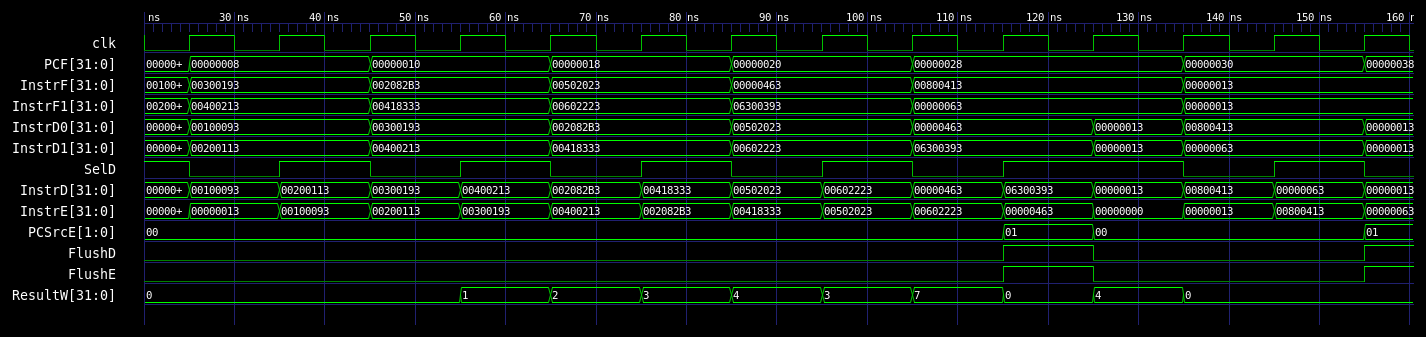
\includegraphics[width=\textwidth]{../img/prog5_dualfetch.png}
\caption{Programa 5, de 20 a 160~ns.}
\label{fig:p5}
\end{figure}

En la Figura~\ref{fig:p5} se ve el ritmo del Dual Fetch. A los 30~ns, Decode tiene el par \sig{0x00} (\sig{InstrD0 = addi x1}, \sig{InstrD1 = addi x2}) y, al mismo tiempo, Fetch ya está leyendo el par \sig{0x08} (\sig{InstrF = addi x3}, \sig{InstrF1 = addi x4}). Con \sig{SelD = 0} sale \sig{addi x1}; a los 40~ns, con \sig{SelD = 1}, sale \sig{addi x2}, mientras el PC y el par de Fetch esperan. A los 50~ns entra el par \sig{0x08} a Decode y \sig{PCF} salta de \sig{0x08} a \sig{0x10}. El patrón se repite cada dos ciclos: un par leído y decodificado, dos instrucciones emitidas.

El salto aparece a los 110~ns, cuando entra el par \sig{0x20} con el \sig{beq} en el slot~0 y \sig{addi x7, 99} en el slot~1. El \sig{beq} se emite primero y a los 120~ns se resuelve tomado en EX (\sig{PCSrcE = 01}) justo cuando se está emitiendo \sig{addi x7}. \sig{FlushE} la anula (a los 130~ns \sig{InstrE} vale 0) y \sig{FlushD} limpia el par. A los 140~ns entra el par destino (\sig{addi x8} y \sig{beq fin}) y todo sigue en orden.

\begin{nota}{Un error que encontramos con este programa}
Al revisar la simulación vimos que, si un salto se tomaba mientras se emitía el slot~0, el PC no saltaba: solo se actualizaba cuando \sig{SelD = 1}, y el destino se perdía. Lo corregimos permitiendo que el PC se actualice también cuando hay un salto tomado (\sig{en = ~StallF & (SelD | FlushD)}), y agregamos al testbench la verificación del destino después de cada salto, que con la versión anterior falla.
\end{nota}

% =====================================================================
\section{Conclusiones}
% =====================================================================

El pipeline de cinco etapas ejecuta correctamente el subconjunto RV32I que soporta y resuelve los tres riesgos del pipeline: forwarding desde MEM y WB, un ciclo de stall ante load-use y la anulación de dos instrucciones en cada salto tomado. Las pruebas automáticas fueron clave: gracias a ellas encontramos dos errores, el flush que faltaba en \sig{jalr} y la pérdida del destino del salto en el Dual Fetch, que con una revisión visual de las waveforms habrían sido fáciles de pasar por alto.

La base del Dual-Issue ya está: Fetch y Decode trabajan con pares de instrucciones y el Register File tiene los cuatro puertos de lectura y dos de escritura que se van a necesitar. La vía 1 ya tiene su registro ID/EX y su ALU. Para E2 queda lo más interesante: completar esa vía hasta WB, la Issue Unit que decida si dos instrucciones pueden salir juntas (dependencias RAW dentro del par y recursos compartidos de memoria y branch) y el forwarding entre vías.

\appendix
\section{Cómo reproducir las pruebas en Vivado}

El código entregado tiene dos carpetas: \sig{Single_Issue}, con la arquitectura A, y \sig{Dual_Issue}, con el avance hacia B. Dentro de cada una hay una carpeta por programa con su código Assembly, su archivo \sig{.mem} y su testbench (Tabla~\ref{tab:repro}). Los programas 1 a 4 también pasan sin cambios en \sig{Dual_Issue}.

\begin{table}[htbp]
\centering
\small
\caption{Archivos de cada prueba.}
\label{tab:repro}
\begin{tabular}{l l l l l}
\toprule
\textbf{Programa} & \textbf{Código} & \textbf{Carpeta} & \textbf{Testbench} & \textbf{Programa cargado} \\
\midrule
1 (ISA)        & \sig{Single_Issue} & \sig{Programa1_ISA}        & \sig{tb_isa.v}        & \sig{isa.mem} \\
2 (Forwarding) & \sig{Single_Issue} & \sig{Programa2_Forwarding} & \sig{tb_forwarding.v} & \sig{forwarding.mem} \\
3 (Stalling)   & \sig{Single_Issue} & \sig{Programa3_Stalling}   & \sig{tb_stalling.v}   & \sig{stalling.mem} \\
4 (Flushing)   & \sig{Single_Issue} & \sig{Programa4_Flushing}   & \sig{tb_flushing.v}   & \sig{flushing.mem} \\
5 (Dual Fetch) & \sig{Dual_Issue}   & \sig{Programa5_DualFetch}  & \sig{tb_dualfetch.v}  & \sig{dualfetch.mem} \\
\bottomrule
\end{tabular}
\end{table}

\textbf{Una sola vez, para crear el proyecto:}

\begin{enumerate}
  \item Crear un proyecto RTL nuevo en Vivado.
  \item Agregar como \textit{design sources} todos los archivos \sig{.v} de la carpeta \sig{Single_Issue} (de \sig{adder.v} a \sig{top.v}). Para el Programa~5 se crea otro proyecto igual, pero con los \sig{.v} de \sig{Dual_Issue}.
\end{enumerate}

\textbf{Para cada programa de la Tabla~\ref{tab:repro}:}

\begin{enumerate}[resume]
  \item Agregar como \textit{simulation sources} el testbench del programa y su \sig{.mem} asociado. Por ejemplo, para el Programa~1: \sig{Programa1_ISA/tb_isa.v} e \sig{Programa1_ISA/isa.mem}.
  \item Hacer clic derecho sobre ese testbench y elegir \textit{Set as Top}.
  \item Ejecutar \textit{Run Simulation} $\to$ \textit{Run Behavioral Simulation}.
  \item Revisar la consola Tcl: el testbench se detiene solo e imprime \sig{PASS} o \sig{FAIL}.
  \item Cerrar la simulación (\textit{Close Simulation}) antes de pasar al siguiente programa.
\end{enumerate}

En la ventana de waveform aparecen directamente \sig{PCF}, \sig{InstrF} a \sig{InstrW} y las señales de la Hazard Unit, porque el testbench las declara en su nivel superior. Es normal que Vivado muestre un aviso como \sig{WARNING: file Programa1_ISA/isa.mem could not be opened}: el testbench primero busca el \sig{.mem} dentro de la carpeta del programa y, al no encontrarlo ahí, carga la copia que Vivado deja en su carpeta de simulación.

\end{document}
